%----------------------------------------------------------------------------------------
%   CV - 黎子豪
%   Refined typography: bilingual CJK + Latin, refined hierarchy & spacing
%----------------------------------------------------------------------------------------
\documentclass[a4paper,11pt]{article}

%----------------------------------------------------------------------------------------
%   FONTS & SPACING TUNING
%----------------------------------------------------------------------------------------
\usepackage{fontspec}
\usepackage{xeCJK}

% Latin: EB Garamond (Serif) for classic elegance in body
\IfFontExistsTF{EB Garamond}{%
  \setmainfont{EB Garamond}[
    Ligatures      = TeX,
    Numbers        = OldStyle,
  ]
}{%
  \setmainfont{Baskerville}[
    BoldFont       = Baskerville SemiBold,
    ItalicFont     = Baskerville Italic,
    BoldItalicFont = Baskerville SemiBold Italic,
  ]
}

% Sans: Helvetica Neue for clean, modern headings
\setsansfont{Helvetica Neue}[
  UprightFont = * Light,
  BoldFont    = * Medium,
  ItalicFont  = * Italic,
]

% CJK Main: Songti SC (Serif) pairs perfectly with Garamond
\setCJKmainfont{Songti SC}[
  UprightFont = *,
  BoldFont    = * Bold,
  ItalicFont  = Kaiti SC,
]

% CJK Sans: PingFang SC for headings
\setCJKsansfont{PingFang SC}[
  UprightFont = * Regular,
  BoldFont    = * Medium,
]

% Advanced CJK typography spacing
\xeCJKsetup{
  CJKecglue = {\hskip 0.25em plus 0.08em minus 0.05em}, % wider CJK-Latin spacing
  PunctStyle = kaiming, % Elegant punctuation spacing
}

%----------------------------------------------------------------------------------------
%   PACKAGES
%----------------------------------------------------------------------------------------
\usepackage[top=2cm, bottom=2cm, left=1.8cm, right=1.8cm]{geometry} % slightly more breathable margins
\usepackage[usenames,dvipsnames]{xcolor}
\usepackage{graphicx}
\usepackage{tabularx}
\usepackage{enumitem}
\usepackage{titlesec}
\usepackage{fontawesome5}
\usepackage{tikz}
\usepackage{parskip}
\usepackage{microtype}

\newcolumntype{C}{>{\centering\arraybackslash}X}
\newcolumntype{R}{>{\raggedleft\arraybackslash}X}
\renewcommand{\arraystretch}{1.2} % Better spacing for tabular environments

%----------------------------------------------------------------------------------------
%   COLORS
%----------------------------------------------------------------------------------------
\definecolor{accent}{HTML}{1A365D}      % Deep Oxford Blue (very professional)
\definecolor{linkcolour}{HTML}{2B6CB0}  % Slightly brighter blue for links
\definecolor{doubangreen}{HTML}{2A8C3F} % Douban-style green
\definecolor{fbblue}{HTML}{1877F2}      % official Facebook blue
\definecolor{rule}{HTML}{E2E8F0}        % Soft slate gray for rules
\definecolor{muted}{HTML}{64748B}       % Elegant slate gray for secondary text
\definecolor{body}{HTML}{1E293B}        % Slate near-black for softer contrast
\definecolor{pagebg}{HTML}{F7F7F5}      % Light grey-white page background

\usepackage{pagecolor}
\pagecolor{pagebg}

\color{body}

% Display font for the Latin name line — Playfair Display preferred.
\IfFontExistsTF{Playfair Display}{%
  \newfontfamily{\namefont}{Playfair Display}[LetterSpace=4.0]
}{%
  \IfFontExistsTF{EB Garamond}{%
    \newfontfamily{\namefont}{EB Garamond}[LetterSpace=4.0]
  }{%
    \newfontfamily{\namefont}{Baskerville}[LetterSpace=4.0]
  }%
}

\usepackage[unicode, draft=false]{hyperref}
\hypersetup{
  colorlinks,
  breaklinks,
  urlcolor  = linkcolour,
  linkcolor = linkcolour,
}

%----------------------------------------------------------------------------------------
%   SECTION STYLE
%----------------------------------------------------------------------------------------
\titleformat{\section}
  {\sffamily\bfseries\Large\color{accent}}
  {}{0em}{}
  [\vspace{-3pt}{\color{rule}\titlerule[0.8pt]}]
\titlespacing*{\section}{0pt}{18pt}{8pt} % More white space before/after sections

%----------------------------------------------------------------------------------------
%   LIST STYLES
%----------------------------------------------------------------------------------------
\setlist[itemize]{
  nosep,
  leftmargin = 1.4em,
  itemsep    = 4pt,
  parsep     = 1pt,
  topsep     = 5pt,
  label      = {\color{accent}\scriptsize\raisebox{0.25ex}{$\circ$}}, % clean hollow circle
}

%----------------------------------------------------------------------------------------
%   LINE SPACING
%----------------------------------------------------------------------------------------
\linespread{1.2} % Better line height for mixed CJK and English
\setlength{\parskip}{3pt}

%----------------------------------------------------------------------------------------
%   ENTRY MACROS
%----------------------------------------------------------------------------------------
% \entryhead{title}{date}
\newcommand{\entryhead}[2]{%
  \par\vspace{6pt}
  \noindent\begin{tabularx}{\linewidth}{@{}X r@{}}
    {\large\bfseries\color{body}#1} & {\small\color{muted}\sffamily #2} \\
  \end{tabularx}\par\vspace{2pt}
}

% \entrymeta{role / venue / PI}{right-side note (optional)}
\newcommand{\entrymeta}[2]{%
  \noindent\begin{tabularx}{\linewidth}{@{}X r@{}}
    {\normalsize\itshape\color{body} #1} & {\small\color{muted}\textbf{#2}} \\
  \end{tabularx}\par\vspace{4pt}
}

%----------------------------------------------------------------------------------------
\begin{document}
\pagestyle{empty}

%----------------------------------------------------------------------------------------
%   HEADER — photo (left) + name & contacts (right)
%----------------------------------------------------------------------------------------
\noindent
\begin{minipage}[c]{0.20\textwidth}
  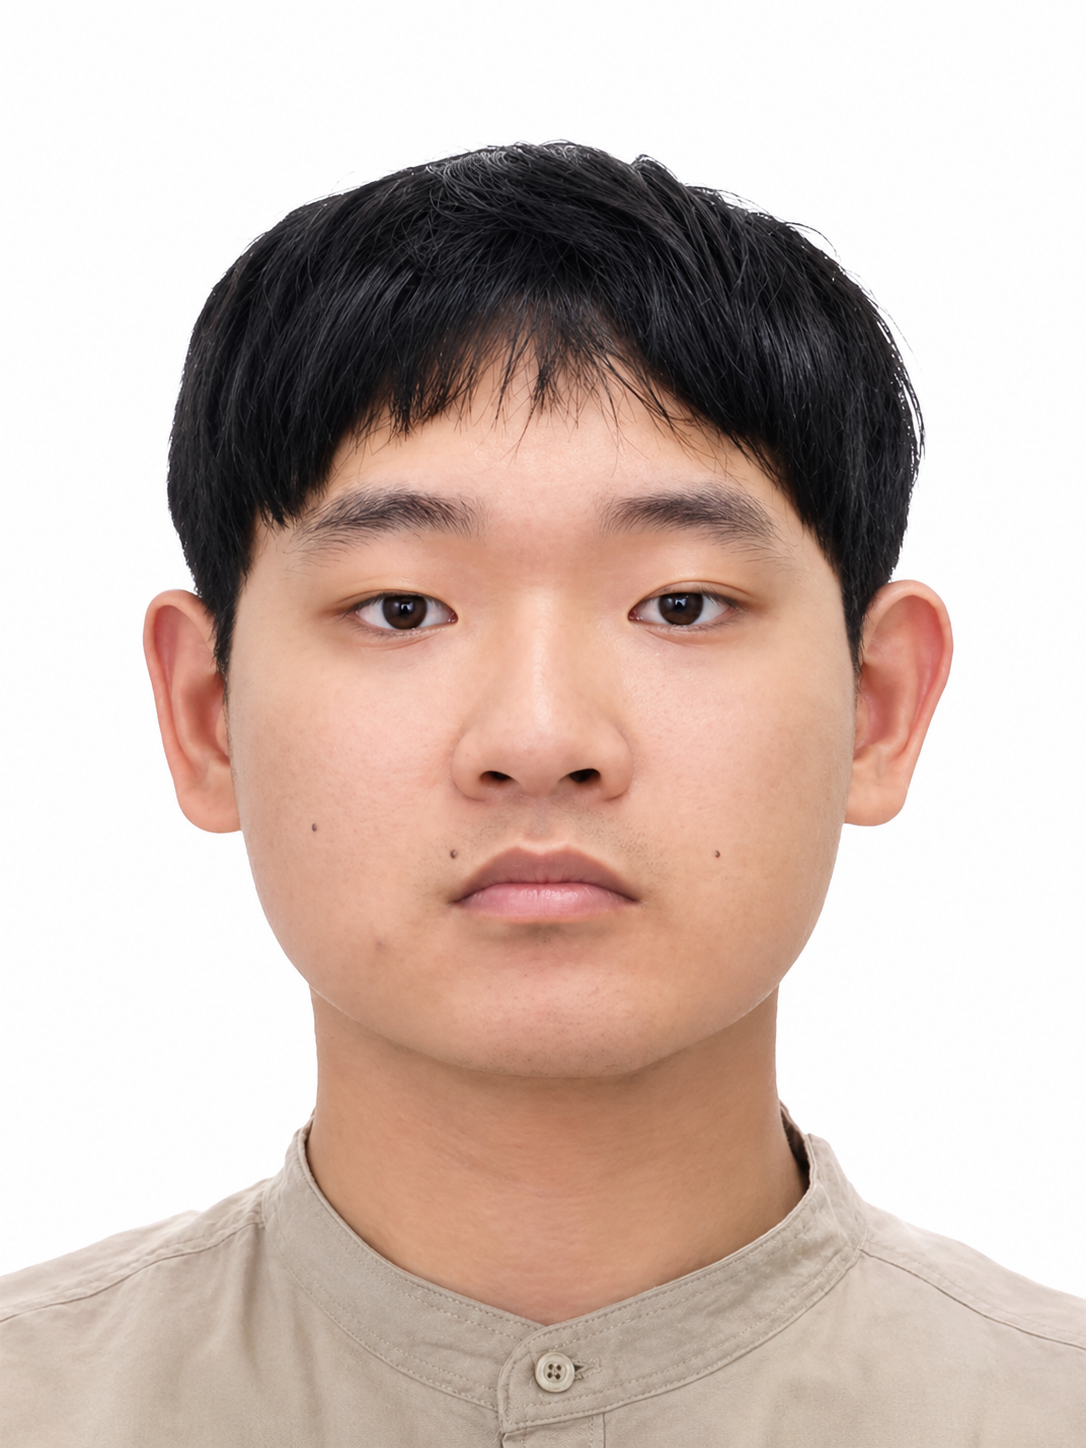
\includegraphics[width=\linewidth]{photo-for-cv.png}
\end{minipage}%
\hfill
\begin{minipage}[c]{0.78\textwidth}
\begin{center}
\vspace{25pt}
% Name — refined serif with subtle letter-spacing
{\namefont\fontsize{40}{44}\selectfont\color{accent} Li Zihao}\\[6pt]
{\sffamily\normalsize\color{muted}黎\,子\,豪 \quad|\quad Journalism \& Communication Studies}\\[12pt]
% Top row: 3 primary contacts
{\sffamily\small\color{linkcolour}%
  \href{https://chiselli.com}{\faGlobe\,\,chiselli.com}\hspace{2.2em}%
  \href{mailto:lizihao2023@lzu.edu.cn}{\faEnvelope[regular]\,\,lizihao2023@lzu.edu.cn}\hspace{2.2em}%
  \href{https://github.com/MiShenng}{\faGithub\,\,MiShenng}%
}\\[8pt]
% Bottom row: 2 secondary social contacts, centered beneath
{\sffamily\small%
  \href{https://www.douban.com/people/chiselli}{\color{doubangreen}\faBookOpen}\,\,{\color{linkcolour}\href{https://www.douban.com/people/chiselli}{Douban\,\,|\,\,豆瓣}}\hspace{2.6em}%
  \href{https://www.facebook.com/chiselli}{\color{fbblue}\faFacebookF}\,\,{\color{linkcolour}\href{https://www.facebook.com/chiselli}{Facebook}}%
}
\end{center}
\end{minipage}

\vspace{6pt}

%----------------------------------------------------------------------------------------
%   EDUCATION
%----------------------------------------------------------------------------------------
\section{教育经历}

\entryhead{兰州大学 \normalfont\textcolor{muted}{\,/\,Lanzhou University}}{Sep.\ 2023\,--\,present}
\entrymeta{新闻学学士\,\,Bachelor of Journalism}{GPA \textbf{4.07}\,/\,5.0}
\begin{itemize}
  \item \textbf{相关课程：}新媒体用户分析、传播心理学、媒介批评、传播学研究方法、数据新闻、传播学概论
\end{itemize}

\entryhead{台湾师范大学 \normalfont\textcolor{muted}{\,/\,National Taiwan Normal University}}{Aug.\ 2025\,--\,Dec.\ 2025}
\entrymeta{交换生\,\,Exchange Student}{GPA \textbf{3.9}\,/\,4.0}
\begin{itemize}
  \item \textbf{相关课程：}视觉文化与传播、新媒介与社会、社会科学研究方法
\end{itemize}

%----------------------------------------------------------------------------------------
%   PUBLICATIONS
%----------------------------------------------------------------------------------------
\section{会议论文}

\entryhead{Framing}{AEJMC 2026}
\entrymeta{Li, Z.}{[\,\href{https://some-link.com}{\faGlobe}\,]}
\begin{itemize}
  \item 讲讲怎么做
  \item 讲讲有什么用
\end{itemize}

%----------------------------------------------------------------------------------------
%   WORKING PAPERS
%----------------------------------------------------------------------------------------
\section{Working Papers \& Research in Progress}

\entryhead{Scripted Rage and Patriotic Camouflage: The Algorithmic Commodification of Han Chauvinism in Chinese Platform}{IAMCR 2026}
\entrymeta{Jiang, J.\textsuperscript{*}}{[\,\href{https://some-link.com}{\faGlobe}\,]}
\begin{itemize}
  \item say something
  \item say something
\end{itemize}

%----------------------------------------------------------------------------------------
%   RESEARCH EXPERIENCE
%----------------------------------------------------------------------------------------
\section{研究经历}

\entryhead{中央高校基本科研项目 \normalfont\textcolor{muted}{\,/\,Fundamental Research Funds for Central Universities}}{Sep.\ 2024\,--\,May 2025}
\entrymeta{say something}{\textbf{研究助理}}
\begin{itemize}
  \item Proposed the ``Frame--Emotion Dual-Track Interaction Model,'' demonstrating how frames and emotional appeals co-evolve to shape perception.
  \item Used LLMs (DeepSeek) and the CARER model for large-scale analysis, revealing systematic patterns by media ownership and region.
  \item Constructed a 48-year longitudinal corpus, including manual digitization of pre-2008 print and microfiche archives.
\end{itemize}

\entryhead{Ukrainian Wartime Poetry Project}{Jun.\ 2025\,--\,Jan.\ 2026 \,(expected)}
\entrymeta{PI: Prof.\ Amelia Glasser, University of California, San Diego}{\textbf{Research Assistant}}
\begin{itemize}
  \item Built a Chrome extension and data pipeline to systematically collect and de-duplicate 4{,}000+ Ukrainian Facebook poems, turning an ad-hoc workflow into a reproducible corpus for annotation and analysis.
  \item Co-developed an advanced annotation manual for Ukrainian pronouns, specifying referent categories (self, intimate, local, nation, state, enemy, etc.), ``we''-inclusivity, syntactic and semantic roles, discourse functions, and stratified sampling protocols for 400--600 tokens.
  \item Annotating and modeling shifts in poetic voice and polyphony (monologic vs.\ mediated vs.\ choral) together with collocation networks (2014--2025) to trace how person perspective and national-identity vocabularies transform across wartime phases.
\end{itemize}

\entryhead{The Symbiotic Development of Digital Nomads and Rural Communities}{Mar.\ 2024\,--\,Jul.\ 2024}
\entrymeta{PI: Prof.\ Rui Wang, Communication University of China}{\textbf{Research Assistant}}
\begin{itemize}
  \item Modeled interpersonal communication networks through 20 in-depth interviews, identifying pathways for virtual identity formation and community integration.
\end{itemize}

\entryhead{Big Data Project on Global Opinions}{Jan.\ 2024\,--\,Jan.\ 2026 \,(expected)}
\entrymeta{PI: Prof.\ Ting Zhou, Communication University of China}{\textbf{Research Assistant}}
\begin{itemize}
  \item Executed sentiment analysis on 500+ Western media articles regarding China's ``Two Sessions'' for China's National News Agency.
  \item Monitored credibility risks for foreign social media accounts, producing weekly analytical briefings.
\end{itemize}

\entryhead{Desire to Remain Young: An Investigation of Elderly Matchmaking in China}{Mar.\ 2023\,--\,Jun.\ 2023}
\entrymeta{2024 Paper Data Content Annual Case Collection Award}{\textbf{Research Project Developer}}
\begin{itemize}
  \item Collected and coded a qualitative dataset from 22 in-depth interviews to analyze identity and desire in matchmaking contexts.
  \item Designed an award-winning interactive data story website, implementing a full-stack solution for dynamic user-profile comparison.
\end{itemize}

%----------------------------------------------------------------------------------------
%   WORK EXPERIENCE
%----------------------------------------------------------------------------------------
\section{Selected Work Experience}

\entryhead{China Telecom}{Jan.\ 2022\,--\,Mar.\ 2022}
\entrymeta{Event Operations Intern}{}
\begin{itemize}
  \item Analyzed real-time social media data (Weibo, WeChat) to model user-engagement patterns and public-opinion trends.
  \item Performed large-scale comment analysis to identify key audience demographics and public sentiment, guiding content development.
\end{itemize}

\entryhead{iFeng}{Sep.\ 2023\,--\,Dec.\ 2023}
\entrymeta{News Editing Intern}{[\,\href{https://some-link.com}{\faGlobe}\,]}
\begin{itemize}
  \item Authored and published press releases on emerging technology for iFeng.com, covering major industry events.
  \item Developed video scripts for the \textit{ifengTech} column and conducted daily public-opinion monitoring, providing analytical briefings.
\end{itemize}

%----------------------------------------------------------------------------------------
%   ACADEMIC SERVICE
%----------------------------------------------------------------------------------------
\section{Academic Service}

\noindent\begin{tabularx}{\linewidth}{@{}X r@{}}
  \textbf{Peer Reviewer}\,\,\,{\small\color{muted}International Communication Association (ICA)} & {\small\color{muted}\itshape Nov.\ 2024} \\[3pt]
  \textbf{Peer Reviewer}\,\,\,{\small\color{muted}International Political Science Association (IPSA)} & {\small\color{muted}\itshape Nov.\ 2024} \\
\end{tabularx}

%----------------------------------------------------------------------------------------
%   COMMUNITY
%----------------------------------------------------------------------------------------
\section{Community \& Volunteer Engagement}

\noindent\begin{tabularx}{\linewidth}{@{}X r@{}}
  \textbf{Outstanding Volunteer}\,\,\,{\small\color{muted}The Third Belt and Road Forum for International Cooperation} & {\small\color{muted}\itshape Oct.\ 2023} \\[3pt]
  \textbf{Outstanding Volunteer}\,\,\,{\small\color{muted}China International Fair for Trade in Service (CIFTIS)} & {\small\color{muted}\itshape Sep.\ 2023} \\[3pt]
  \textbf{Volunteer Teacher}\,\,\,{\small\color{muted}Guanghua Foundation Voluntary Teaching Programme} & {\small\color{muted}\itshape Jun.\ 2023} \\
\end{tabularx}

%----------------------------------------------------------------------------------------
%   AWARDS
%----------------------------------------------------------------------------------------
\section{Selected Awards \& Honors}

\noindent\begin{tabularx}{\linewidth}{@{}X r@{}}
  \textbf{Outstanding Undergraduate Thesis Award} \,{\small\color{muted}(University-Level)} & {\small\color{muted}\itshape May 2025} \\[3pt]
  \textbf{Paper Data Content Annual Case Collection Award} & {\small\color{muted}\itshape Jun.\ 2024} \\[3pt]
  \textbf{Second-Class Scholarship} \,{\small\color{muted}(University-Level)} & {\small\color{muted}\itshape Nov.\ 2024} \\[3pt]
  \textbf{Meritorious Student} \,{\small\color{muted}(University-Level)} & {\small\color{muted}\itshape Sep.\ 2022\,--\,Sep.\ 2024} \\[3pt]
  \textbf{Practical Scholarship} \,{\small\color{muted}(University-Level)} & {\small\color{muted}\itshape Oct.\ 2023} \\
\end{tabularx}

%----------------------------------------------------------------------------------------
%   SKILLS
%----------------------------------------------------------------------------------------
\section{Skills}

{\renewcommand{\arraystretch}{1.4}
\noindent\begin{tabularx}{\linewidth}{@{}>{\bfseries\color{accent}}l X@{}}
  Programming      & Python {\small\color{muted}(Pandas, Scikit-learn, PyTorch, NLTK, spaCy)}, R, Web {\small\color{muted}(HTML, CSS, JavaScript)} \\[2pt]
  Analytical Tools & SPSS, NVivo, Tableau, ECharts \\[2pt]
  NLP\,/\,ML       & BERT, SBERT, LDA, and other transformer-based architectures \\[2pt]
  Production       & \LaTeX, Microsoft Office Suite, Adobe Creative Suite {\small\color{muted}(Premiere, Photoshop)} \\
\end{tabularx}%
}

\vfill
\begin{center}{\scriptsize\color{muted}Last updated:\ \today}\end{center}

\end{document}
